% Expanded development studies with provisional model judgments.
\section{Source eligibility and experimental interpretation}

A role field identifies a transport role; it does not establish who authored a
message. Inspection of partial annotation disagreements revealed scheduled
automation prompts inside records marked as user messages. The source filter
had omitted this envelope format. The same audit identified mixed records
containing pasted material, injected instructions, and command or interface
context. Some mixed records contain genuine user requests. Their complete
contents cannot be treated as independent human-authored observations without
further attribution.

The expanded extraction produced 24,497 candidate spans from 6,425 selected
source records. Before fitting a model, we stopped annotation and preserved its
requests, responses, and unresolved attempts. Whole-source quarantine removed
1,362 records and their 15,385 candidates. A further 35 eligible candidates had
issued annotation attempts without validated outcomes and were excluded rather
than silently retried. The corrected pool contains 9,077 candidates. Completed
valid annotations are reused under a separate, frozen protocol. This correction
followed inspection of partial training labels and is an adaptive development
decision. Remaining authorship is unverified; whole-source quarantine also
excludes some genuine text embedded in mixed records.

The broader source graph links 35 of the earlier replay study's 42 primary
development candidates to components represented in training. A separate check
of complete source records finds automated or mixed envelopes behind 34 of the
42 candidates, including 32 scheduled automation messages. The same issue
affects 196 of 485 training candidates. The earlier measurements remain
historical regression diagnostics. Filtering the evaluation rows alone would
leave affected training in place. The corrected study preserves the existing
conservative component assignments and reserved confirmation groups.

\subsection{Corrected-source learning curves}

The corrected annotation protocol produced agreement on 5,979 of 9,077 candidates;
3,098 still require review. These are agreements between models, with no
independent human labels. Finalization removed seven repeated or cross-partition
candidate copies, leaving 5,548 training rows and 424 development rows. The
conservative source graph places the training rows in one connected component
and the development rows in thirty components. Of the development rows, 66
belong to previously examined components and 358 to newly allocated development
components. Both slices are development data. Reserved confirmation records
were not read or fitted.

Training retention labels comprise 233 durable, 4,522 temporary, 517 ignore,
and 276 uncertain examples. Development contains 14, 346, 40, and 24 examples
respectively. Of 360 typed development examples, 304 are projects, 31 facts,
24 preferences, and one a routine; behavior and relationship have no support.
The training sources therefore expand volume much more than class diversity.
Agreement filtering and conservative source quarantine can also change the
distribution being measured.

We fitted multinomial logistic heads over a frozen MiniLM encoder at five
natural-source counts: 0, 100, 500, 2,000, and all 3,332 source units. All fits
retain 1,063 original synthetic training examples. Three seeded, nested
source-prefix draws define the intermediate points. Each identical zero-source
and full-source endpoint is fitted once per weighting rule. Unweighted and
inverse-frequency class-balanced fitting yield 22 pairs of heads. The heads
use $C=10$ and at most 1,500 optimizer iterations; every fit converged before
that limit. Candidate context matches the serving contract. All formatted inputs fit its
declared 256-token limit, with no silent truncation.

Temperature is selected separately for each head by development negative
log-likelihood from $\{0.5,0.75,1,1.5,2,3,5\}$. Reporting selective performance
on that same set makes the calibration results optimistic. The fixed joint
acceptance threshold is 0.8. At the full-source endpoints, retention temperature
is 1.5 and type temperature is 1.0 for both weighting rules. Source counts and
fitting costs intentionally vary: this experiment measures data scaling, not
an equal-compute replay advantage.

\begin{figure}[htbp]
\centering
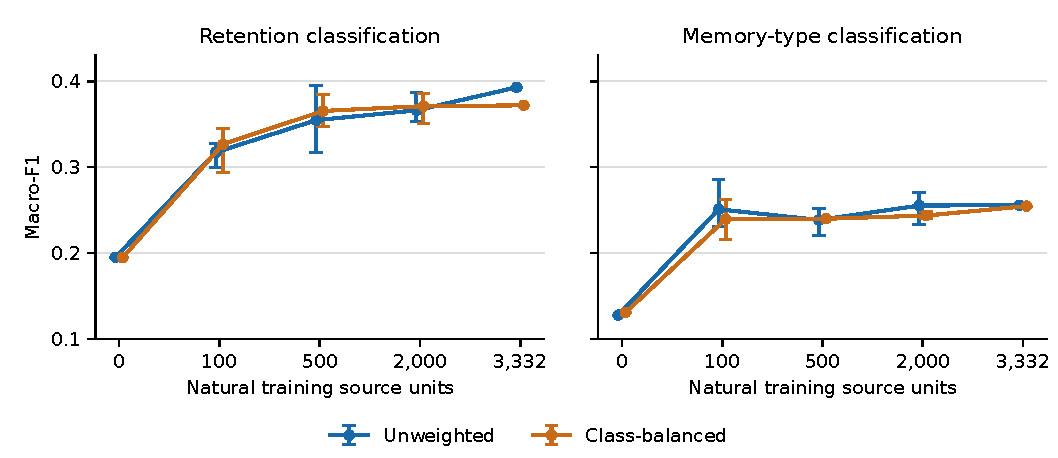
\includegraphics[width=\linewidth]{images/expanded-learning-curves.pdf}
\caption{Development learning curves on provisional labels. Source counts are
shown at equally spaced categorical positions. Points are means and bars are
the ranges of three source-subset draws at intermediate counts, not confidence
intervals. Endpoints contain one fit per weighting rule. Type macro-F1 averages
all six configured classes, assigning zero F1 to the two classes with no
development support; their recall remains unevaluated.}
\label{fig:expanded-curves}
\end{figure}

Unweighted retention macro-F1 increases from 0.195 with synthetic examples
alone to 0.393 at the full-source endpoint (Figure~\ref{fig:expanded-curves}).
That endpoint recovers none of the fourteen durable examples. Class balancing
recovers five, but predicts durable for seventy examples, of which sixty-five
disagree with the provisional labels. Its durable precision is therefore
$5/70=7.1\%$. Higher aggregate agreement does not establish useful durable-memory
admission.

\begin{table}[htbp]
\centering\small
\begin{tabular}{lrrrr}
\toprule
Training rule & Retention F1 & Type F1 & Durable hits & Joint errors/accepted\\
\midrule
Training majority & 0.225 & 0.153 & 0/14 & ---\\
Unweighted & 0.393 & 0.256 & 0/14 & 14/151\\
Class-balanced & 0.372 & 0.255 & 5/14 & 7/28\\
\bottomrule
\end{tabular}
\caption{Full-source development results. F1 is macro-averaged over four
retention or six type classes. The majority labels are selected from training
data only. Joint errors are disagreements with provisional labels among
accepted predictions, with coverage denominators of 424. They are neither
independently reviewed errors nor unsupported-memory counts.}
\label{tab:expanded-classification}
\end{table}

At threshold 0.8, unweighted fitting accepts 151/424 examples (35.6\%) with
14/151 disagreements (9.3\%). Balanced fitting accepts 28/424 (6.6\%) with
7/28 disagreements (25.0\%). The training-majority retention prediction alone
has 81.6\% accuracy, compared with 80.7\% unweighted and 61.3\% balanced
accuracy. Project dominance similarly makes majority type accuracy 84.4\%.
Accuracy therefore obscures substantial minority-class failures.

Encoding 7,035 rows required 384,356 input tokens, 16.1 seconds wall time and
29.1 CPU seconds on the shared local machine. The 22 head fits and their reports
took a summed 2.5 seconds wall time and 2.5 CPU seconds. These totals exclude
source extraction, annotation, model loading, and earlier synthetic generation.
They are not an isolated throughput benchmark. Per-class confusion matrices,
calibration diagnostics, source-subset ranges, and both development slices
accompany the paper as aggregate data.

No classifier is promoted from this comparison. The next development study
should test representation adaptation and loss weighting against these frozen
baselines, while improving independently reviewed class coverage. Increasing
the same source distribution alone does not resolve the observed durable-class
failure or establish a sleep-inspired learning benefit.


\subsection{Retaining synthetic training examples}

A twelve-run development study tested whether retaining original synthetic
training examples reduces forgetting of the designed classification tasks.
Each of four conditions used three seeds and 64 updates of 32 presentations.
Every update contained the same sixteen newer-source examples, eight older or
replayed examples, and eight original synthetic examples. Relative to the
earlier zero-anchor comparison, the synthetic block replaced half of the
older or replayed block. Update counts, model capacity, and padded token shapes
were held fixed. Data composition changed intentionally; actual input tokens,
earlier generation work, and wall time were not matched.

\begin{table}[htbp]
\centering
\small
\begin{tabular}{lrrrr}
\toprule
Condition & Synthetic 0 & Synthetic 8 & Older & Newer \\
\midrule
Ordinary training & 0.710 & 0.980 & 0.547 & 0.248 \\
Repeated examples & 0.811 & 0.975 & 0.333 & 0.155 \\
Paraphrases & 0.697 & 0.978 & 0.333 & 0.155 \\
Recombination & 0.784 & 0.964 & 0.362 & 0.155 \\
\bottomrule
\end{tabular}
\caption{Mean retention-classification macro-F1 over three seeds. The first
two numeric columns compare zero and eight synthetic presentations per update.
The older and newer columns report the eight-anchor runs on the historical
24- and 18-candidate development cohorts. Those cohorts are affected by the
source-authorship and overlap findings above and do not establish independent
human-conversation transfer.}
\end{table}

Synthetic type-classification macro-F1 after the eight-anchor runs ranged from
0.970 to 0.978, and synthetic relationship recall ranged from 0.982 to 1.000.
These results support retaining task coverage during this adaptation exercise.
Neither generated-replay condition exceeded ordinary training on both
historical development measures. They provide no evidence that generated
rehearsal improves factual knowledge retention or reduces unsupported memories.

\section{Visibility of corrections}

Classification agreement does not establish factual retention. A memory system
must also receive the observation that changes an existing fact. Let $I(H)$
denote all information available to a consolidation and answering procedure
after admission and retrieval from history $H$. This includes its initial
memory state and every supplied source, timestamp, and metadata value. It
excludes observations withheld by the host policy.

\begin{samepage}
\begin{proposition}[Indistinguishable omitted corrections]
Suppose two histories $H_0,H_1$ satisfy $I(H_0)=I(H_1)$ but the correct current
answer to the same query is respectively $y_0$ and $y_1$, with $y_0\ne y_1$.
For any procedure whose output depends only on $I(H)$ and randomness independent
of the history, the output distribution is identical in both histories.
Under a uniform mixture of the two histories, if the procedure answers with
probability $a$ and otherwise abstains, its probability of an incorrect answer
is at least $a/2$.
\end{proposition}

\begin{proof}
Equal available inputs and the same distribution of independent randomness
induce the same output law. Write $p(y)$ for the probability of answering $y$.
The total answer probability is $a=\sum_y p(y)$. The probability of a correct
answer under the uniform mixture is
$\tfrac12 p(y_0)+\tfrac12 p(y_1)\leq a/2$ because the two correct values are
distinct. Subtracting correct-answer probability from $a$ gives an error
probability of at least $a/2$. Abstention contributes to neither term.
\end{proof}
\end{samepage}

The proposition is conditional on identical available information. It gives no
empirical error rate and makes no claim about biological consolidation or
learning convergence. It explains why a source-admission policy and the
consolidator need separate evaluation: an omitted correction cannot be recovered
from an unchanged summary alone.

\section{Fictional history diagnostics}

We evaluated two explicitly fictional, two-stage histories with an earlier
state, later corrections, and unchanged facts. Four learned source-selection
policies each supplied six of ten observations per stage. The policies used
ordinary training, repeated examples, source-grounded paraphrases, or
recombination, with three training seeds. An additional all-source reference
supplied ten observations and therefore had a larger source allowance. All
learned conditions shared consolidation-call and retrieval limits. Provider
sampling seeds were not controllable.

The resulting thirty episodes completed the persistence and consolidation
checks. At the later stage, strict memory-only answer counts were 46/54 for
ordinary training, 44/54 for repetition, 42/54 for paraphrases, and 41/54 for
recombination. The all-source reference obtained 52/54. These denominators
contain repeated questions over two templates; they are not independent
conversation samples. Supplying retrieved original observations produced
54/54 later answers in every condition. That result can conceal failures in
source admission because the source reader can access observations omitted from
consolidation.

Six later memories were judged stale. In every case, the source-selection
policy had withheld the correcting observation. The all-source reference had
no stale-current flags in this study. This diagnosis supports testing admission
separately from correction handling; it does not demonstrate an error in the
production consolidator, whose classifier remains advisory.

The original support judge flagged fourteen distinct memory identifiers across
the thirty episodes. Each persisted into the second stage, producing
twenty-eight phase-level flags. All fourteen concern the same employment
instruction pattern. The original fixture treated an instruction to store a
claim as insufficient support. Ordinary memory requests can also communicate
self-reports, so this boundary depends on the intended annotation policy.
The flags cannot be presented as fourteen independent factual inventions.
Original scores remain unchanged. A separate fictional contrast study examines
direct self-reports, ordinary memory requests, explicit fabrication, quotations,
assistant suggestions, negation, and corrections. Its model-written expectations
also require independent human review.

That contrast study used seventeen fixtures with two provider replicates, for
thirty-four cases and thirty-eight consolidation stages. Every consolidation
and semantic-review call returned a valid result. Model review found no
forbidden current claim in twenty-eight checks. Nineteen of twenty required
phase-level claims were present; one quoted employment report about another
person was omitted in one replicate. Direct self-reports and ordinary memory
requests were retained in all six corresponding checks. No model-judged subject
or temporal-scope error occurred. These results qualify the earlier instruction
test and identify an omission to investigate. They do not establish a zero
unsupported-memory rate on natural conversations.

The contrast study used 76 provider calls and 86,134 returned tokens, with
205.1 seconds of summed request time. The database was isolated, its dump was
retained privately, and its container was removed after completion. This study
tested the current consolidation prompt without changing a production policy.

\subsection{Retrieval and answer quality}

For twelve frozen snapshots from the all-source reference, we compared lexical
retrieval with hybrid retrieval using the pinned MiniLM encoder. Both methods
returned at most four memory hits and four original-source windows. Among
seventy-two answerable queries, the prescribed source was present in 71/72
lexical memory lists and 66/72 lexical source lists. Hybrid retrieval returned
it in 72/72 lists for both representations. Source presence does not establish
entailment, attribution, or a correct answer.

Hybrid retrieval also returned memory and source hits for all thirty-six
unanswerable queries. Subsequent model-only semantic review found 52/54 correct
early memory-only answers for hybrid retrieval and 51/54 for lexical retrieval.
Early source-assisted answers were 53/54 for both. Later memory-only results
were 52/54 for both, and later source-assisted results were 54/54. One early
hybrid source-assisted answer supplied the policy-dependent employer claim.
These small development results do not establish a general retrieval advantage
or justify a production-default change.



\subsection{Historical ingestion order}

A separate diagnostic supplies dated fictional observations in chronological
and reverse order. Four fixtures describe changing residence or preference,
each with two provider replicates, for eight episodes and sixteen consolidation
stages. All observations are supplied directly; no classifier selects them.
Source dates also appear in the text. The historical-backfill cases require an
older observation arriving later to preserve the newer current claim.

Model review finds all sixteen required phase-level claims and none of twelve
forbidden current claims. No consolidation, subject-attribution, or temporal-scope
error is recorded in the completed episodes. One database startup attempt failed
before any provider request or persisted row; its failure record was preserved
and the empty database was verified before resuming. This setup failure is
separate from the completed consolidation results.

The diagnostic used 32 returned provider calls, 40,530 tokens and 101.1 seconds
of summed request time. Its expectations and semantic judgments are model-authored,
and the fixtures are fictional. The result supports further testing of dated
imports; it does not measure safety on natural email or establish that arbitrary
historical backfills preserve current beliefs.
